\documentclass[10pt,a4paper]{article}
\usepackage{fontspec,polyglossia}
\setmainlanguage{russian}
\setmainfont{Times New Roman}
\usepackage{amsmath,amssymb,booktabs,tabularx,graphicx}
\usepackage[margin=17mm]{geometry}
\usepackage[hidelinks]{hyperref}
\usepackage{titlesec}
\titleformat{\section}{\large\bfseries}{}{0pt}{}
\titlespacing*{\section}{0pt}{8pt}{4pt}
\setlength{\parindent}{0pt}
\setlength{\parskip}{4pt}
\setlength{\emergencystretch}{3em}
\begin{document}
{\Large\bfseries Проверка MG при сохранении информации в текстовом коде}\par\medskip

29 сентября 2026. Третья ветвь добавлена к тем же десяти сохранённым состояниям: пилот 0 и подтверждающие seeds 1--9. Исходные ветви и их результаты не изменялись.

\textbf{Критерий сохранения кода выполнен в 9/9 подтверждающих seed.} Среди этих seed MG в защищённой ветви выше, чем в ветви с потерей информации, в 9/9; ближе к исходному контролю --- в 9/9. Медианное отношение MG protected/regularized по всем девяти seed --- 1,286. Таблица включает все seed, без отбора по результату.

\section*{1. Какой вопрос проверяем}

Текстовый VAE учится восстанавливать предложения: encoder читает предложение и строит Gaussian-распределение кода, decoder предсказывает слова по предыдущим истинным словам и выборке этого кода. При усилении KL-регуляризации модель может перестать использовать код. Проверяем, различает ли MG потерю информации и сохранение её существенной части при одинаковом внешнем коэффициенте регуляризации.

В каждой тройке \textbf{base} оставляет beta=0,01, \textbf{regularized} меняет beta на 1, \textbf{protected} делает то же изменение с защитой. Все ветви стартуют из одинаковых весов, Adam и состояния генератора после 1024 обновлений. Конец --- 3072 обновления. Основные батчи и латентный шум совпадают.

\textbf{Данные и модель:} Penn Treebank, 6000 обучающих и 256 проверочных предложений; длина 8--24 слова плюс EOS; словарь 2000. Embedding размерности 48, encoder и decoder GRU по 64 скрытых координаты, код размерности 16; всего 276016 параметров. Teacher forcing, без dropout. Adam с шагом 0,001, batch 32, ограничение нормы градиента 5. Исходный loss --- средняя по батчу сумма NLL слов предложения плюс beta, умноженный на KL posterior к стандартному Gaussian prior. Два исходных продолжения переиспользованы из архивов.

\section*{2. Как выбиралась защита}

Сначала на pilot 0 проверены пять дополнительных шагов encoder на каждое обычное обновление. Decoder и общие embedding на внутренних шагах действительно неизменны, включая их Adam-состояния. Поздняя информация составила 0,520 нат против 5,480 до вмешательства; реакция на перестановку --- 0,040 против 0,569. Эта попытка не прошла критерий сохранения кода; она сохранена отдельно и не используется как проверка специфичности MG.

Использован заранее предусмотренный запасной вариант \textbf{free bits}: для каждой из 16 координат считаем средний по батчу KL к prior, заменяем его максимумом с 0,5 нат и суммируем. При этом внешний коэффициент beta равен 1, как в ветви с потерей информации. Это не жёсткое ограничение на информацию: код должен использоваться ради восстановления текста. Выполняется одно обычное обновление Adam на шаг.

Free bits меняет форму функции потерь. Поэтому этот контроль слабее по изоляции причины, чем сохранение исходной функции потерь и дополнительные шаги encoder. Он позволяет сравнить два режима с одинаковым внешним beta, но не устраняет все различия динамики оптимизации.

\textbf{Критерий сохранения кода задан до запусков:} поздние медианы (шаги 2048--3072) взаимной информации и реакции предсказаний на перестановку кода должны каждая составлять не менее половины исходной медианы (шаги 512--1024) и быть хотя бы вдвое выше regularized. Сначала проверялся этот критерий на pilot 0, без расчёта его MG; затем выбранная защита зафиксирована для всех seeds 1--9 независимо от результата MG. Seed с неудачной защитой: нет.

\textbf{Измерения.} Информация --- MC с четырьмя выборками на предложение для смеси 256 posterior (потолок log 256 нат). Реакция на код --- симметризованный KL предсказаний при циклической перестановке распределений encoder между предложениями и согласованном шуме, в нат/токен. Эти проверки выполняются каждые 128 шагов. MG получает только reconstruction NLL/token на первых 16 проверочных предложениях и фиксированном Gaussian noise. Окно 512, сдвиг 128, размерность вложения 20, задержка 1, 20 соседей, Theiler 39; тренд не удаляется. Поздние окна заканчиваются на шагах 2048--3072 и не пересекают развилку.

\newpage

\section*{3. Все тройки и сравнение MG}

\begin{center}\small
\begin{tabularx}{\linewidth}{l>{\raggedright\arraybackslash}X>{\raggedright\arraybackslash}X>{\raggedright\arraybackslash}X>{\raggedright\arraybackslash}X}
\toprule
Seed & Информация reg / prot & Реакция на код reg / prot & MG reg / prot & $R$ \\
\midrule
0 (пилот) & 0,26 / 3,85 & 0,015 / 0,568 & 3,79 / 5,64 & 1,489 \\
1 & 0,21 / 4,03 & 0,005 / 0,598 & 4,59 / 5,49 & 1,196 \\
2 & 0,22 / 3,85 & 0,014 / 0,599 & 4,04 / 5,22 & 1,292 \\
3 & 0,33 / 3,83 & 0,021 / 0,580 & 4,14 / 5,53 & 1,334 \\
4 & 0,47 / 3,97 & 0,038 / 0,609 & 4,21 / 5,19 & 1,234 \\
5 & 0,43 / 4,01 & 0,050 / 0,600 & 4,35 / 5,59 & 1,286 \\
6 & 0,19 / 3,93 & 0,008 / 0,572 & 3,75 / 5,56 & 1,481 \\
7 & 0,58 / 3,95 & 0,048 / 0,620 & 4,36 / 4,98 & 1,143 \\
8 & 0,65 / 3,88 & 0,078 / 0,614 & 4,17 / 4,92 & 1,179 \\
9 & 0,16 / 3,91 & 0,007 / 0,575 & 3,96 / 5,62 & 1,418 \\
\bottomrule\end{tabularx}\end{center}

Все значения --- поздние медианы. $R=\mathrm{MG}_{protected}/\mathrm{MG}_{regularized}$: больше 1 означает более высокий MG при защите. Звёздочка отмечает непрошедший независимый критерий защиты; такие seed не скрыты. Основная статистика исключает pilot 0. По прошедшим критериям seed 95\% bootstrap-интервал медианы R --- [1,179; 1,418] (20000 ресэмплирований пар seed, условно на фиксированном корпусе).

\begin{center}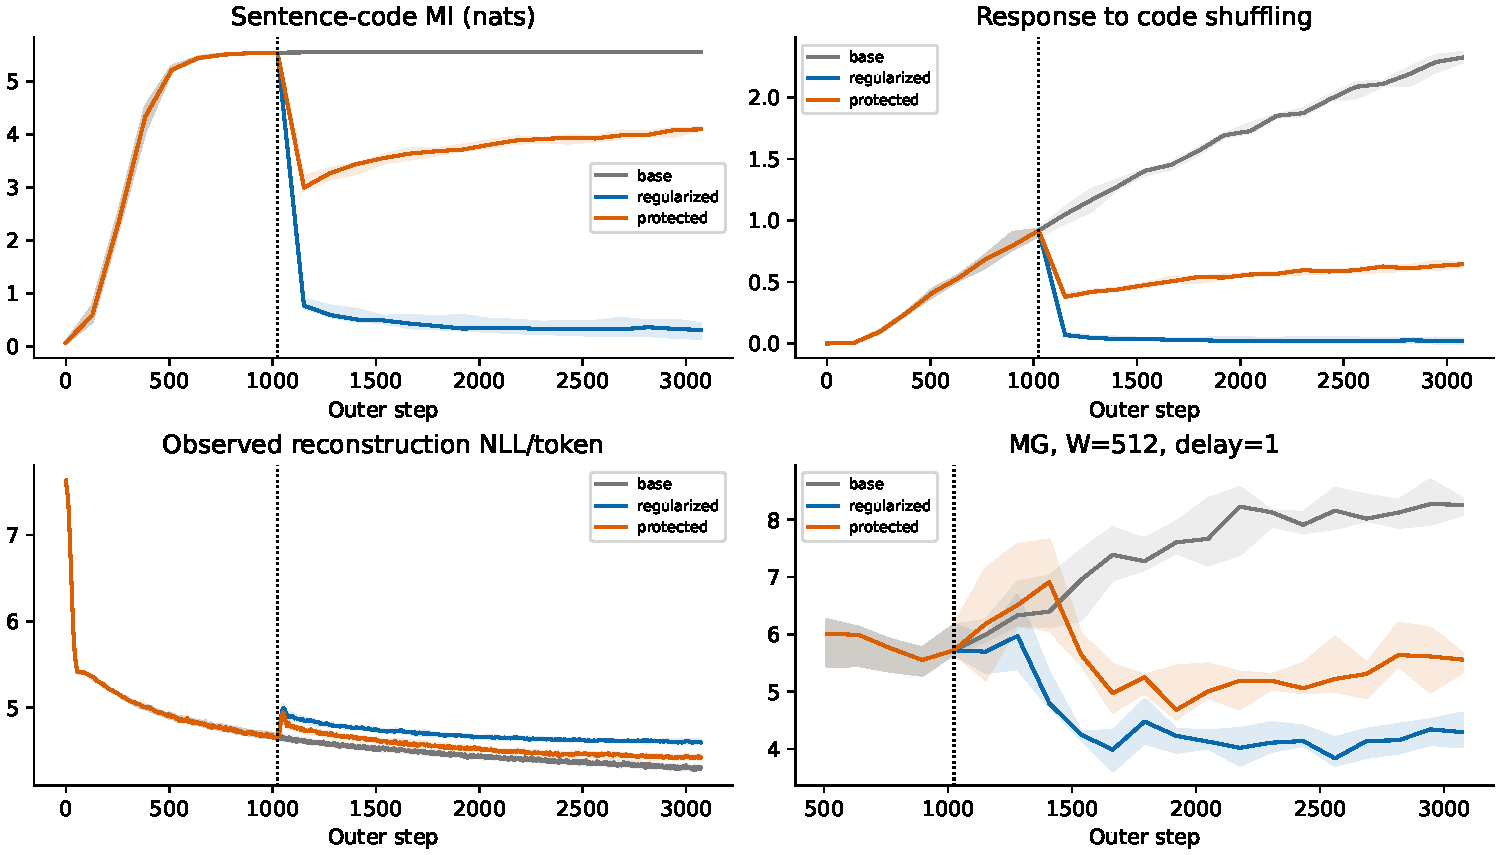
\includegraphics[width=\linewidth,height=.30\textheight,keepaspectratio]{comparison_cohort.pdf}\end{center}

Медиана и межквартильный диапазон по всем seeds 1--9, включая неудачные защиты. Серый --- base, синий --- regularized, оранжевый --- protected. Сверху независимые характеристики кода, снизу наблюдаемый loss и MG. Оси времени одинаковы; дополнительных внутренних обновлений encoder на оси нет.

\textbf{Устойчивость:} W=512, delay=1: медиана R=1,286, R>1 в 9/9; W=256, delay=1: медиана R=1,299, R>1 в 9/9; W=1024, delay=1: медиана R=1,254, R>1 в 9/9; W=512, delay=4: медиана R=1,285, R>1 в 9/9. Это заранее сохранённые дополнительные настройки; основной вариант не менялся. \textbf{Дешёвые альтернативы на том же входе:} стандартное отклонение: отношение protected/regularized 1,302, выше в 9/9; спектральная энтропия: отношение protected/regularized 1,048, выше в 7/9. Преимущество MG перед ними этим контролем не установлено.

\textbf{Граница вывода.} Защита сохраняет значительную, но не всю информацию. Медиана protected/base для MG --- 0,639, regularized/base --- 0,517: полного возвращения к исходному контролю нет. Более высокий MG при защите согласуется с меньшей потерей информации в данной постановке, но free bits также меняет динамику оптимизации. Контроль не доказывает ни точную размерность, ни универсальную причинную специфичность MG. KL и простые статистики loss остаются конкурентами; преимущества в стоимости здесь не заявляем.

Протокол, неудачная попытка encoder5, все финальные веса, диагностические CSV и варианты окон сохранены. Это дополнительные продолжения прежних инициализаций, не новая серия независимых данных.
\end{document}